\documentclass[tikz]{standalone}
%\usepackage{geometry}

%graphics


\usetikzlibrary{shapes.geometric, shapes.multipart, arrows, calc, through,intersections}
\usepackage[caption=false,font=footnotesize]{subfig}

\tikzset{
    pics/mig/.style = {
        code = {%
        \coordinate (-center) at (0, 0);
        \coordinate (-north) at (0, .5cm);
        \coordinate (-south) at (0,-.5cm);
        \coordinate (-se) at (310:.5cm);
        \coordinate (-sw) at (230:.5cm);
        \draw[line width=1mm](0,0)circle[radius=.5cm];
        }
    },
}
\begin{document}

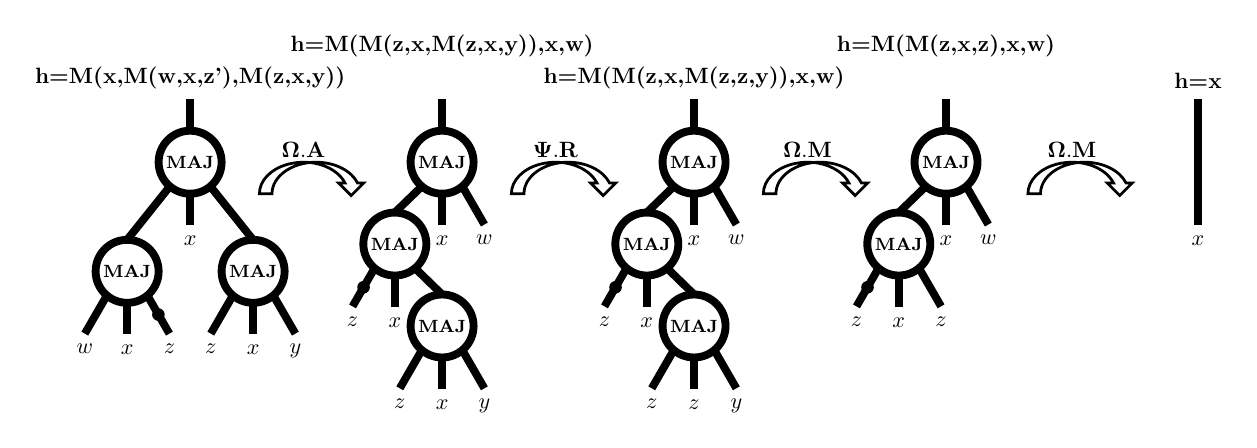
\begin{tikzpicture}[scale=0.8,transform shape,line width=1mm]

\begin{scope}[xshift=-4cm]
\pic(m1) at (0,0) {mig};
\node at(m1-center){\textbf{\footnotesize MAJ}};
\pic(m2) at (240:2) {mig};
\node at(m2-center){\textbf{\footnotesize MAJ}};
\pic(m3) at (300:2) {mig};
\node at(m3-center){\textbf{\footnotesize MAJ}};

\draw(m1-north)-- ++(0,.5cm) node[above]{\textbf{h=M(x,M(w,x,z'),M(z,x,y))}};
\draw(m1-south)-- ++(0,-.5cm) node[below]{\textbf{$x$}};
\draw(m1-sw) -- (m2-north);
\draw(m1-se) -- (m3-north);

\draw(m2-sw) -- ++(240:0.7)node[below]{\textbf{$w$}};
\draw(m2-south)-- ++(0,-.5cm)node[below]{\textbf{$x$}};
\draw(m2-se) -- ++(300:0.7)node[below]{\textbf{$z$}};
\fill ($(m2-se)+(300:0.35)$) circle[radius=1mm];

\draw(m3-sw) -- ++(240:0.7)node[below]{\textbf{$z$}};
\draw(m3-south)-- ++(0,-.5cm)node[below]{\textbf{$x$}};
\draw(m3-se) -- ++(300:0.7)node[below]{\textbf{$y$}};
\end{scope}

\begin{scope}[xshift=-2.7cm,yshift=-0.5cm,line width=1pt]
\draw(0,0)arc[start angle=180,delta angle=-160, x radius=7mm, y radius=5mm] -- ++(1mm,0) -- ++(-2mm,-2mm) -- ++(-2mm,2mm) -- ++(1mm,0) arc[start angle=20,delta angle=160, x radius=7mm, y radius=5mm] -- cycle;
\node at (5mm,7mm) {$\mathbf{\Omega.A}$};
\end{scope}

\begin{scope}
\pic(m1) at (0,0) {mig};
\node at(m1-center){\textbf{\footnotesize MAJ}};
\pic(m2) at (240:1.5) {mig};
\node at(m2-center){\textbf{\footnotesize MAJ}};
\pic(m3) at (0,-2.6) {mig};
\node at(m3-center){\textbf{\footnotesize MAJ}};

\draw(m1-north)-- ++(0,.5cm) node[above=5mm]{\textbf{h=M(M(z,x,M(z,x,y)),x,w)}};
\draw(m1-south)-- ++(0,-.5cm) node[below]{\textbf{$x$}};
\draw(m1-sw) -- (m2-north);
\draw(m1-se)-- ++(300:0.7)node[below]{$w$};

\draw(m2-south)-- ++(0,-.5cm)node[below]{$x$};
\draw(m2-sw)-- ++(240:0.7)node[below]{$z$};
\fill ($(m2-sw)+(240:0.35)$) circle[radius=1mm];

\draw(m2-se)-- (m3-north);
\draw(m3-south)-- ++(0,-.5cm)node[below]{$x$};
\draw(m3-sw)-- ++(240:0.7)node[below]{$z$};
\draw(m3-se)-- ++(300:0.7)node[below]{$y$};
\end{scope}

\begin{scope}[xshift=1.3cm,yshift=-0.5cm,line width=1pt]
\draw(0,0)arc[start angle=180,delta angle=-160, x radius=7mm, y radius=5mm] -- ++(1mm,0) -- ++(-2mm,-2mm) -- ++(-2mm,2mm) -- ++(1mm,0) arc[start angle=20,delta angle=160, x radius=7mm, y radius=5mm] -- cycle;
\node at (5mm,7mm) {$\mathbf{\Psi.R}$};
\end{scope}

\begin{scope}[xshift=4cm]
\pic(m1) at (0,0) {mig};
\node at(m1-center){\textbf{\footnotesize MAJ}};
\pic(m2) at (240:1.5) {mig};
\node at(m2-center){\textbf{\footnotesize MAJ}};
\pic(m3) at (0,-2.6) {mig};
\node at(m3-center){\textbf{\footnotesize MAJ}};

\draw(m1-north)-- ++(0,.5cm) node[above]{\textbf{h=M(M(z,x,M(z,z,y)),x,w)} };
\draw(m1-south)-- ++(0,-.5cm) node[below]{\textbf{$x$}};
\draw(m1-sw) -- (m2-north);
\draw(m1-se)-- ++(300:0.7)node[below]{$w$};

\draw(m2-south)-- ++(0,-.5cm)node[below]{$x$};
\draw(m2-sw)-- ++(240:0.7)node[below]{$z$};
\fill ($(m2-sw)+(240:0.35)$) circle[radius=1mm];

\draw(m2-se)-- (m3-north);
\draw(m3-south)-- ++(0,-.5cm)node[below]{$z$};
\draw(m3-sw)-- ++(240:0.7)node[below]{$z$};
\draw(m3-se)-- ++(300:0.7)node[below]{$y$};
\end{scope}

\begin{scope}[xshift=5.3cm,yshift=-0.5cm,line width=1pt]
\draw(0,0)arc[start angle=180,delta angle=-160, x radius=7mm, y radius=5mm] -- ++(1mm,0) -- ++(-2mm,-2mm) -- ++(-2mm,2mm) -- ++(1mm,0) arc[start angle=20,delta angle=160, x radius=7mm, y radius=5mm] -- cycle;
\node at (5mm,7mm) {$\mathbf{\Omega.M}$};
\end{scope}

\begin{scope}[xshift=8cm]
\pic(m1) at (0,0) {mig};
\node at(m1-center){\textbf{\footnotesize MAJ}};
\pic(m2) at (240:1.5) {mig};
\node at(m2-center){\textbf{\footnotesize MAJ}};

\draw(m1-north)-- ++(0,.5cm) node[above=5mm]{\textbf{h=M(M(z,x,z),x,w)}};
\draw(m1-south)-- ++(0,-.5cm) node[below]{\textbf{$x$}};
\draw(m1-sw) -- (m2-north);
\draw(m1-se)-- ++(300:0.7)node[below]{$w$};

\draw(m2-south)-- ++(0,-.5cm)node[below]{$x$};
\draw(m2-sw)-- ++(240:0.7)node[below]{$z$};
\fill ($(m2-sw)+(240:0.35)$) circle[radius=1mm];
\draw(m2-se)-- ++(300:0.7)node[below]{$z$};
\end{scope}

\begin{scope}[xshift=9.5cm,yshift=-0.5cm,line width=1pt]
\draw(0,0)arc[start angle=180,delta angle=-160, x radius=7mm, y radius=5mm] -- ++(1mm,0) -- ++(-2mm,-2mm) -- ++(-2mm,2mm) -- ++(1mm,0) arc[start angle=20,delta angle=160, x radius=7mm, y radius=5mm] -- cycle;
\node at (5mm,7mm) {$\mathbf{\Omega.M}$};
\end{scope}

\begin{scope}[xshift=12cm]
\draw(0,1)node[above]{\textbf{h=x}} -- (0,-1)node[below]{$x$};
\end{scope}




\end{tikzpicture}

\end{document}
